\subsection{Self-Play}
\label{selfplay}
\begin{comment}

- Dota 2 openai
    - https://openai.com/five/
    - https://openai.com/blog/openai-baselines-ppo/
    
- phan paper training 1 - agents develop motor skills
- \cite{selfplay-heinrich}  many real-world applications are in principle games

- schach?
- go?
- dota?
- physical openai

"if you arent really good - your opponent isnt either. if you are getting better - your opponent gets better" - perfect curriculum

"agent that you train in self play is useful for external task"

https://www.youtube.com/watch?v=BJi6N4tDupk

supervised learning - limited by dataset - creates ceiling of how far it can go
\end{comment}

%\inline{TDGammon --> Go was für verbesserungen? viel übernommen, beides modelbased. Go wesentlich komplizierter als TDGammon. Dota 2 modelfree, 5 neuronale netze, kooperation usw.}
In October 2015, the Al AlphaGo defeated European champion Fan Hui in the Go game. In March 2016, 18-time international champion Lee Sedol was beaten by AlphaGo's successor \cite{GoalphaGosilver2017mastering}. 
AlphaGo was initially trained with the help of supervised learning, fed with moves from professional players.
The problem with supervised learning is that the available data set usually implies an upper limit for the learning performance. Reinforcement learning, on the other hand, learns from its own experience and can advance into areas that humans may not be able to fathom. So the AI AlphaGo has managed to achieve superhuman performance and defeat the best Go players in the world, but may not have reached its full potential yet.\\
As a result, Deepmind developed a program called AlphaGo Zero that learned exclusively through self-play "tabula rasa". This means that the agent did not know any sample moves from expert players or could compare his own with them. Only the rules of the game were given to the agent at the beginning. Starting with random game moves, AlphaGo became the best currently existing Go player in the world, beating the previously mentioned champion AlphaGo 100-0. But not only Go, also Chess and the japanese version of it, "shogi", was mastered by the algorithm \cite{chessSilver2017mastering,GoalphaGosilver2017mastering}. \\
\\
%\inline{überarbeiten!}
Self-play means that the agent always plays against a copy of itself.
Deepminds AlphaZero uses Monte-Carlo Tree Search (MCTS) \cite{montecarlobrowne2012survey} and a deep neural network that estimates the probability of winning the current player has from the active position.
A deep neural network $f_\theta$ with parameters $\theta$ is used. The neural network gets as input the raw board presentation $s$ from the position and the history and outputs move probabilities and a value $(\textbf{p}, v) = f_\theta (s)$, where

\begin{description}

    \begin{itemize}
        \item The vector of move probabilities \textbf{p} represents the probability of each possible move (including \textit{pass} where the player forgoes his move), $p_a = Pr(a|s)$. 
        
        \item The value $v$ is a scalar rating that estimates the win probability of the current player from position $s$.\inline{variable ändern!}
    \end{itemize}

\end{description}

This neural network assumes the roles of policy network and value network (section \ref{reinforcement}) in a single environment.  The parameters $\theta$ are updated so that the similarity of the policy vector \textbf{$p_t$} to the search probability \textbf{$\pi_t$} (in the Monte-Carlo Tree Search) is maximized and the error between the predicted winner $v_t$ and the actual game winner $z$ is minimized. More precisely, the parameter $\theta$ is determined by gradient descent with a loss function $l$ that sums over mean-squared error and cross-entropy losses respectively \cite{GoalphaGosilver2017mastering}.
MCTS is a predictive search that allows you to efficiently search for the best move possible. Using a minmax algorithm, the tree would quickly gain depth in a complex game like Go and would therefore not be suitable. Also, the actual value of each action can be approximated by performing several random simulations.
\\
\\
%TDgammon
Self-play is not a completely new field of research. Already in 1992 Gerald Tesauro \cite{TDGammontesauro1992practical,TD2Gammontesauro1995temporal} developed a neural net, which learned to play backgammon on world champion level. The game-learning "TD-Gammon" is a neural net that trains itself to be an evaluation-function and learn from the outcome of each game.
27 years later, on april 13, 2019, OpenAI "Five" was the first AI to beat a world champion in an esports game named Dota 2. Afterwards, OpenAI Five was made available to all Dota 2 players as opponent or team partner - the potentially largest deployment of a highly professional deep learning agent with whom people can knowingly interact, winning 99.4\% of its games versus humans \cite{dotaOpenAI2019Jun}.\\ 
\\
Dota 2 is a highly complex game, much more complex than Go. While model-based reinforcement learning was applied in backgammon and go, a model-free approach is pursued here. Dota 2 is not turn-based, but a real-time strategy game, the individual agent can not be sure before his decision what impact and reward his action will have. OpenAI Five consists of a team of five artificial neural networks, which started with no knowledge. A huge difference to the achievements of AlphaGo is that the neural networks must not only compete, but also cooperate to maximize their reward. From the bots' point of view, Dota 2 is a structure of 20,000 (compared to chess' 8x8) numbers that reflect what a human eye would see. Another essential difference to board games like chess or Go is that Dota 2 has hidden information - only a fraction of the current game board is known to the AI. 180 years of gameplay each day has played the AI against copies of itself, consuming the processing power of 128,000 CPU cores and 256 GPUs. For every game frame, OpenAI's training system called "Rapid" awards a positive reward when something good has happened and a negative reward when something bad has happened. OpenAI's Proximal Policy Optimization \cite{ppoSchulman2019Mar} is then applied and results in actions immediately before a positive reward being rated better than those prior to a negative reward \cite{dotaOpenAI2019Jun}.\\
\\
The OpenAI team has also discovered that self-play with simulated agents can lead to learning physical skills such as ducking, faking, kicking, catching, etc. without prior knowledge \cite{environmentBansal2017Oct}. At the beginning of the training a dense reward (\textit{exploration reward}) is given for some steps to teach the agent basic motor skills like running or standing. Then the agents get reward for specific actions. For example, two agents stand on a round platform and have to try to push each other off the platform (environment "Sumo" \ref{fig:sumo}). The humanoid agent learned to bump with his head and dodge the attacking opponent at the edge of the platform to let him run into nowhere. \\
The movement strategies learned in this adversarial environment are not only useful for competition, but can also be transferred to other scenarios. For example, the agent trained in sumo was disturbed with wind forces while the goal was to stand upright \cite{environmentBansal2017Oct}.
\begin{figure}[H]
  \centering
    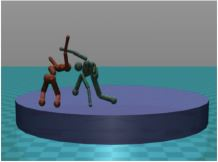
\includegraphics[width=0.5\textwidth]{adversarial_learning/images/sumo.JPG}
    \label{fig:sumo}
    \caption{Illustration of a competitive environment called \textit{Sumo} \cite{environmentBansal2017Oct}}
\end{figure}

%evtl checker by samuel



